% !TEX program = lualatex

\documentclass[a4paper,12pt]{article}

\usepackage[tmargin=20mm,bmargin=20mm,lmargin=30mm,rmargin=20mm]{geometry} % Formato de página

\usepackage[output-decimal-marker={,}]{siunitx} % Unidades del SI
    \sisetup{per-mode = fraction, fraction-function=\sfrac}

\usepackage{csquotes} % Usado por biblatex
\usepackage[
    backend = biber,
    style = apa,
    sortcites,
    url = true
    ]{biblatex} % Citas y referencias bibliográficas
    \addbibresource{includes/bibliography.bib} % Base de datos de referencias bibliográficas

\usepackage{graphicx}  % Define \includegraphics
    \graphicspath{{./images/}} % Define \graphicspath{{dir1}{dir2}} para incluir imágenes que estén en los directorios dir1 y dir2

\usepackage{multicol} % Separación en columnas
    \setlength\columnsep{18pt}

\usepackage[spanish]{babel}  % Traducciones y abreviaturas
\usepackage{amssymb}  % Símbolos y tipografía matemáticos
\usepackage{amsmath}  % Formato y estructura matemáticos
\usepackage[colorlinks=false, pdfborder={0 0 0}]{hyperref}  % Define \url{} para hipervínculos
\usepackage{fancyhdr}  % Encabezado y pie
\usepackage{pdfpages} % Define \includepdf
\usepackage{float} % Entorno para imágenes
\usepackage{enumitem} % Etiquetas para \begin{enumerate}
% \usepackage{fontspec} % Define \setmainfont{Times New Roman} (requiere LuaLatex)
%     \setmainfont{Times New Roman} % (requiere LuaLatex)
\usepackage{mathptmx}  % Documento con Times New Roman
% COMANDOS DE FORMATO
\newcommand{\concept}[1]{\vspace{2ex} \textbf{#1}} % Subtítulos sin jerarquía
\newcommand{\captionSpace}{-0.8cm} % Espacio entre figuras y pie de foto
\newcommand{\bq}[1]{``#1''} % #1 entre comillas (#1 between quotes)
\newcommand{\sub}[2]{{{#1}_\textsl{{#2}}}} % #1 subíndice #2 (Usado cuando #2 es $texto$)

\begin{document}

\includepdf{./images/MDLI_cover.pdf}
\renewcommand\spanishtablename{Tabla}
\vspace*{3\baselineskip}

\begin{center}
\textbf{\fontsize{14pt}{16pt}\selectfont Evaluación subjetiva de la cancelación activa de ruido en auriculares}

\textbf{Malvicino, Maximiliano Raúl}
\end{center}

\section{Fundamentación e introducción}

Los dispositivos portátiles, como smartphones y tablets, son ampliamente utilizados por todos los grupos de edad.
Los jóvenes los usan, así como las personas mayores. Sirven para muchas aplicaciones diferentes, como escuchar música o hacer llamadas y conferencias.
La contaminación acústica en la via pública, vehículos de transporte, sitios de construcción, o instalaciones industriales afecta la calidad de la experiencia de escucha de los usuarios \parencite{Carlettia2008}.

Existen dos formas de reducir el ruido. La reducción pasiva usa materiales porosos para disminuir el ruido por absorción. Pero su implementación en auriculares es voluminosa, costosa e ineficaz en bajas frecuencias. La reducción activa usa el principio de superposición para cancelar las ondas sonoras del ruido.
Los sistemas pasivos no son eficientes en bajas frecuencias ya que, debido a su naturaleza constructiva, no es posible fabricar material absorbente para sonidos cuyas longitudes de onda superen el tamaño de los auriculares.
La cancelación activa (ANC) ofrece una solución prometedora, ya que según \textcite{Cui2003} resulta efectiva para frecuencias menores a $500 \, \si{\hertz}$ complementándose muy bien con los métodos pasivos.
Consiste en un sistema que utiliza el principio de superposición para eliminar el ruido no deseado.
Detecta el ruido no deseado con un micrófono, genera una señal de \bq{anti-ruido} con la misma amplitud pero en fase opuesta, y combina esta señal con el ruido, lo que resulta en la cancelación de ambos sonidos.

Acorde a \textcite{Kuo1999}, es importante que el sistema ANC sea digital. Esto implica que las señales se muestreen y procesen en tiempo real utilizando sistemas de procesamiento de señales digitales.
Para esto se usa un algoritmo de filtro adaptativo que ajusta las características del anti-ruido generado de manera que se minimice el error entre la señal deseada y la cancelada.
El algoritmo adaptativo más comúnmente utilizado en el control activo de ruido es el algoritmo de mínimos cuadrados medios (LMS, por sus siglas en inglés), el cual se realiza mediante un filtro transversal.
En un filtro transversal, la señal de entrada se divide en múltiples caminos, cada uno de los cuales está ponderado por un coeficiente. Estos coeficientes son ajustados para lograr la respuesta deseada del filtro \parencite[][16-18]{Widrow1985}.

Este estudio se centra en la evaluación de la cancelación activa a través de pruebas subjetivas en los oyentes para determinar la efectividad de la ANC, la percepción de la reducción del ruido y la existencia de posibles interferencias destructivas que alteren la señal deseada.
Esto nos permitirá comprender mejor cómo los usuarios perciben y utilizan la ANC en su vida cotidiana, así como identificar áreas de mejora en el diseño y desarrollo de esta tecnología.

En la sección \ref{sec:objectives}, se determinan los procedimientos a seguir para lograr el objetivo.
La sección \ref{sec:background} pretende establecer una base teórica del funcionamiento de la tecnología en cuestión, y asimismo analizar estudios previos.
Luego se detalla el diseño de la investigación, que comienza en la sección \ref{sec:variables} estableciendo las variables que se van a estar manipulando.
\textcite{Ang2017} sugiere fuertemente que es necesario considerar entornos con ruido real en estudios futuros para obtener una evaluación más precisa de los auriculares ANC.
Por este motivo, en la sección \ref{sec:generatedNoise} se proponen diferentes fuentes de ruido.
Para concluir el diseño de la investigación, en la sección \ref{sec:test} se describe la metodología para llevar a cabo el test subjetivo.
Finalmente, en las secciones \ref{sec:validation} y \ref{sec:results} se realiza la validación de las pruebas y el análisis de los resultados respectivamente.

\section{Objetivos general y específicos}
\label{sec:objectives}

Como objetivo general, se procura evaluar si la ANC cumple con su función de reducir el ruido ambiental sin producir interferencias que afecten la calidad del sonido.

\concept{Objetivos específicos:}

\begin{itemize}[label=\textbullet]
    \item Generar fragmentos de audio que representen las señales deseadas por los usuarios de auriculares y grabaciones de ruido de fondo de posibles situaciones de escucha.

    \item Seleccionar y preparar el recinto donde se llevarían a cabo las pruebas auditivas, así como el equipamiento a utilizar.

    \item Determinar el orden y el nivel SPL que tendrán los fragmentos de señales deseadas y el ruido de fondo en el punto de escucha y realizar el test subjetivo.

    \item Buscar posibles repercusiones de la ANC en la calidad del sonido.

    \item Determinar rango de nivel de ruido de fondo para el cual el sistema ANC cumple su función de suprimir el ruido de fondo.
\end{itemize}

\section{Marco teórico y estado del arte}
\label{sec:background}

Existen sistemas digitales que emplean conversores AD-DA para procesar la señal y generar la cancelación, y sistemas analógicos que utilizan circuitos electrónicos convencionales.

\subsection{ANC analógicos}

Un micrófono que es colocado fuera del auricular capta el ruido ambiental antes de que llegue al oído del usuario.
Esta señal de ruido se interpreta como aquella que debe ser cancelada.
Se genera una señal de polaridad invertida. A esta señal se le aplica un retardador para compensar el tiempo que tarda el ruido en llegar desde el punto donde se ubica el micrófono hasta el oido.
Finalmente, la señal resultante se añade directamente a la música antes de que llegue al oído del usuario.
El esquema de la figura \ref{fig:Kotlicki2016} a continuación representa el sistema.

\begin{center}
    \includegraphics[width=\linewidth]{images/analog_ANC.png}
\end{center}
\vspace{\captionSpace}
\begin{figure}[H]
    \caption{Diagrama de bloques por \textcite{Kotlicki2016}.}
    \label{fig:Kotlicki2016}
\end{figure}

\subsection{Filtros adaptativos}

Un algoritmo LMS (Least Mean Square, por sus siglas en inglés) es un método adaptativo utilizado para ajustar los coeficientes de un filtro digital con el objetivo de minimizar el valor cuadrático medio de una señal de error. Este proceso de minimización se realiza mediante la actualización iterativa de los coeficientes del filtro basándose en el error actual y las entradas del filtro.

\textcite{Rees2006} mencionan varias variaciones del LMS, incluyendo el \bq{filtered-X LMS} (FXLMS), que es una versión adaptada para aplicaciones de control activo de ruido, y que tiene en cuenta la respuesta del sistema (o planta) a través del cual la señal de control es aplicada. Los siguientes son los algoritmos propuestos.

Command-FXLMS ajusta la señal de error hacia un valor de comando dado, en lugar de cero, para controlar el espectro objetivo a una sola frecuencia. Aunque es robusto a errores de amplitud en el modelo de la planta, requiere un esfuerzo de control excesivo cuando la señal de comando está desfasada respecto a la señal de perturbación.

Internal Model FXLMS busca reducir el esfuerzo de control al asegurarse de que la señal de comando y la señal de perturbación estén lo más alineadas en fase posible. Aunque mejora en términos de esfuerzo de control, es muy sensible a errores de amplitud en el modelo de la planta cuando la señal de comando es mucho mayor que la de perturbación.

Phase Scheduled Command-FXLMS (PSC-FXLMS) combina las fortalezas de los dos algoritmos anteriores. Ajusta la fase de la señal de comando según la fase de la perturbación modelada, mientras que su amplitud es fijada independientemente, lo que limita la influencia de errores de magnitud en el modelo de la planta. Sin embargo, es susceptible a errores de fase cuando la amplitud del comando es grande comparada con la perturbación.

\textcite{Chang2007} proponen un algoritmo llamado algoritmo NFXLMS (Neural-based Filtered-X Least Mean Square) que supera al algoritmo FXLMS en la cancelación de ruido no lineal y de banda ancha, y que mejora la convergencia del algoritmo.
La figura \ref{fig:Chang2007} que sigue muestra un esquema de la red neuronal empleada.

\begin{center}
    \includegraphics[width=\linewidth]{images/NFXLMS.png}
\end{center}
\vspace{\captionSpace}
\begin{figure}[H]
    \caption{Arquitectura de red neuronal \textcite[][3]{Chang2007}.}
    \label{fig:Chang2007}
\end{figure}

La capa de entrada está compuesta por nodos que representan las señales de entrada al sistema.
Cada nodo en esta capa corresponde a una característica o parámetro del sistema que se utiliza para modelar y controlar el ruido no deseado.
En el artículo, mencionan que la red propuesta utiliza 4 nodos de entrada, lo que significa que hay 4 parámetros de entrada que se utilizan para caracterizar el ruido y el entorno.
La capa oculta realiza los cálculos y procesamientos intermedios de la red neuronal.
Cada nodo en esta capa toma como entrada la combinación lineal de los valores de salida de los nodos en la capa de entrada, multiplicados por los pesos correspondientes, y aplica una función de activación no lineal a esta suma ponderada.
En el caso del algoritmo NFXLMS, esta capa oculta consta de 6 nodos, como se menciona en el artículo.
En la capa de salida, cada nodo toma como entrada la combinación lineal de los valores de salida de los nodos en la capa oculta, multiplicados por los pesos correspondientes, y aplica una función de activación no lineal. En el algoritmo NFXLMS, esta capa de salida consta de un solo nodo.

Hay dos tipos de sistemas que usan filtros adaptativos: con retroalimentación y de avance.
Los sistemas de control de avance detectan una señal de ruido de referencia, mientras que en los sistemas de retroalimentación esta señal de referencia se desconoce \parencite{Salmasi2011}.

\subsection{ANC con retroalimentación}

En un ANC digital de retroalimentación, se utiliza un micrófono colocado dentro del auricular para capturar el sonido combinado de la música y el ruido externo que llega al oído del usuario.
Esta señal combinada se compara con la señal de audio deseada, y cualquier diferencia se interpreta como ruido que debe ser cancelado.
Se genera una señal de anti-ruido que se agrega a la señal de audio para cancelar el ruido percibido.

El principio básico del ANC adaptativo es estimar el ruido principal que se va a cancelar y usarlo como señal de referencia $x(n)$ para el filtro adaptativo $W(z)$. Como se muestra en la figura \ref{fig:Kuo2018}, la señal secundaria $y(n)$ se calcula a partir de la señal de error $e(n)$ medida por el sensor de error para sintetizar la señal de referencia $x(n)$. Los coeficientes del filtro $W(z)$ se actualizan mediante el algoritmo de mínimos cuadrados filtrados (FXLMS) en el tiempo $n$.

\begin{center}
    \includegraphics[width=0.9\linewidth]{images/feedback_ANC.png}
\end{center}
\vspace{\captionSpace}
\begin{figure}[H]
    \caption{Diagrama de bloques por \textcite[][3]{Kuo2018}.}
    \label{fig:Kuo2018}
\end{figure}

Los sistemas ANC tienen una latencia inherente entre la adquisición del ruido y la emisión de la señal de cancelación \parencite{Liebich2016}.

La señal de ruido ambiental es atenuada pasivamente por los auriculares y percibida como $d'(t)$ dentro del canal auditivo.
Para cancelar esta perturbación, el controlador crea una señal de cancelación que interfiere con $d'(t)$ dejando la señal de error acústico $e'(t) = S(s) \, D(s) - T(s) \, N(s)$, donde $D(s)$ es la señal de ruido ambiental que se quiere cancelar, $N(s)$ representa el ruido de medición, (es decir, cualquier ruido adicional que puede afectar la detección de la señal de ruido), y $S(s)$ y $T(s)$ son funciones de sensibilidad y de sensibilidad complementaria.

Pero en los sistemas de control reatroalimentados se debe verificar la \bq{ecuación del dilema fundamental} que implica que no es posible minimizar simultáneamente $S(s)$ y $T(s)$, ya que $S(s) + T(s) = 1$.
Ante esta situación, estudios como el de \textcite{Liebich2016} investigan controladores de retroalimentación fija, proponiendo la síntesis $\mathcal{H}_\infty$ de sensibilidad mixta.

\subsection{ANC de avance (o retroalimentación directa)}

En un ANC digital con feedforward, el micrófono no se coloca dentro del auricular, sino que se sitúa fuera del mismo, capturando el sonido ambiental antes de que llegue al oído del usuario.
Esta señal capturada se compara con la señal de audio deseada y se cancela la diferencia.
El objetivo es que la señal de anti-ruido cancele el ruido antes de que llegue al oído, de modo que el usuario solo perciba la señal de audio deseada.

Los algoritmos tradicionales usan modelos complejos del ruido de fondo y grandes estructuras de filtro de control, lo que puede ser lento para adaptarse y computacionalmente intensivo.
\textcite{Pawelczyk2000} utiliza solo una estimación del retardo discreto del ruido de fondo, lo que acelera significativamente el procesamiento y reduce la sensibilidad a los cambios el ruido de fondo.
Su algoritmo utiliza principalmente bancos de Phase Shifter para controlar el ruido de banda estrecha de manera efectiva con menos parámetros en comparación con los filtros tradicionales.
En vez de un filtro LMS, utiliza mínimos cuadrados retardados (DLMS).
Los resultados demuestran la efectividad del algoritmo propuesto que proporciona una rápida convergencia y un control efectivo del ruido, aunque se base en un modelo simplificado del ruido de fondo.

\section{Diseño de la investigación}

La cancelación activa en auriculares es una tecnología ampliamente utilizada que pretende mejorar la experiencia auditiva al reducir el ruido ambiental. Sin embargo, la efectividad puede variar significativamente según el diseño del auricular, la calidad del hardware y las preferencias individuales del usuario. Este estudio investiga la percepción de la eficacia de la aplicación a través de un enfoque experimental subjetivo. Se expone a participantes voluntarios a diferentes condiciones de ruido y música mientras usan auriculares. Se les pide que evalúen la calidad del sonido, la reducción de ruido percibida y su nivel de satisfacción con la experiencia auditiva.

En esta investigación se plantea un diseño experimental de alcance correlacional en el cual las siguientes variables se ven involucradas.

\subsection{Variables}
\label{sec:variables}

\begin{itemize}[label=\textbullet]
    \item Uso o no de ANC (objetiva, categórica, independiente).

    \item Nivel de ruido de fondo generado (objetiva, continua, independiente).

    \item Nivel de ruido de fondo percibido por individuo usando auriculares con ANC (subjetiva).

    \item Calidad del sonido percibida por un individuo usando auriculares con ANC (subjetiva).
\end{itemize}

\subsection{Ruido generado}
\label{sec:generatedNoise}

\textcite[][3]{Kuo2018} proponen utilizar sonido natural en lugar de ruido blanco para el modelado de la vía secundaria.
Por lo tanto, se consideran como potenciales fuentes de ruido que puedan afectar la experiencia de los usuarios de auriculares aquellas provenientes del tráfico.

El ruido del tráfico suele tener un espectro de frecuencias amplio, predominando en las bajas y medias frecuencias hasta 1000 $\si{\hertz}$, debido al ruido de los motores y el contacto de los neumáticos con la carretera.
En tráfico terrestre el nivel de potencia (SWL) puede llegar a ser de hasta 100 \si{\deci \bel} y depende de la velocidad y la aceleración de las fuentes \parencite{Can2010}.

Para el caso de aplicación de esta investigación, los sujetos se encuentran inmersos en un área urbana cerca de las fuentes de ruido.
Con lo cual, se espera que algunos ruidos percibidos sean impulsivos y que haya ruido de fondo constante, debido a fuentes lejanas.

Para simular una situación de contaminación sonora, se propone grabar con un micrófono de medición señales de 1 minuto de duración en distintos puntos. Luego, se tomarán fragmentos de los 10 segundos que tengan la información sonora más relevante y representativa de cada situación.
Se propone realizar grabaciones de ruido de fondo que representen la siguiente situación: sujeto escuchando música en un colectivo que recorre una calle transitada.

Para garantizar una situación de control, es imprescindible que el recinto donde se lleve a cabo el experimento tenga un nivel de ruido de fondo de $15 \, \si{\deci \bel}$ SPL menor que el nivel del ruido emitido por el sistema de monitoreo en el punto de escucha.

\subsection{Diseño de prueba subjetiva: Encuesta y muestra}
\label{sec:test}

El test subjetivo consiste en una prueba auditiva para evaluar la efectividad de la cancelación activa comparando la percepción de diferentes usuarios de auriculares.

Según la norma BS.1284-2 de \textcite{ITU1284-2}, se determina que la muestra deberá contar con al menos 10 individuos expertos ya sea por conocimiento en el campo o por entrenamiento auditivo.
Asimismo, la muestra deberá contar con al menos 20 individuos no expertos.

En una primera instancia se le pide al sujeto que brinde sus datos demográficos y se le pregunta si tiene conocimientos en el campo.
Luego, se lo hace escuchar por medio de los auriculares una señal de 10 segundos perteneciente a un fragmento musical.
De manera simultánea, eventualmente se reproduce por un sistema de monitoreo la señal de ruido correspondiente a la situación dada en la sección \ref{sec:generatedNoise}.

Se diseña una encuesta para que el individuo registre las apreciaciones dadas en la tabla \ref{tab:appreciations}.

\begin{table}[ht]
\centering
\begin{tabular}{|c|c|c|}
  \hline
  \textbf{Variable} & \textbf{1} & \textbf{2} \\
  \hline
  Nivel de ruido de fondo & Poco ruido & Mucho ruido \\
  \hline
  Calidad del sonido & Baja calidad & Alta calidad \\
  \hline
\end{tabular}
\caption{Posibles apreciaciones de cada sujeto.}
\label{tab:appreciations}
\end{table}

En el siguiente enlace \url{https://forms.gle/DxoRxnZtbvwvkUyB9} se puede realizar una encuesta de prueba, idéntica a la que respondería cada sujeto.

El sujeto va a realizar 4 escuchas en un orden aleatorio.
En cada una se va a variar el nivel del ruido de fondo generado y se va a activar y desactivar el sistema ANC del auricular. Se pueden identificar entonces los siguientes 4 casos posibles.

\begin{table}[ht]
\centering
\begin{tabular}{|c|c|c|}
  \hline
  \textbf{Escucha} & \textbf{Estado de ANC} & \textbf{Ruido generado} \\
  \hline
  Caso 1 & Apagado & Sin ruido generado \\
  \hline
  Caso 2 & Apagado & Con ruido generado \\
  \hline
  Caso 3 & Encendido & Sin ruido generado \\
  \hline
  Caso 4 & Encendido & Con ruido generado \\
  \hline
\end{tabular}
\caption{Casos posibles de escucha.}
\label{tab:cases}
\end{table}

\section{Validación de las pruebas}
\label{sec:validation}

% Si el sujeto percibe baja calidad sonora en los casos 1 o 2, o si percibe mucho ruido en los casos 1 o 3, será excluido por respuestas inconsistentes.

\section{Análisis de los resultados: Aplicaciones estadísticas}
\label{sec:results}

% 

\section{Conclusiones}

En primer lugar, se espera que las pruebas subjetivas permitan determinar la efectividad percibida de la ANC en la reducción del ruido ambiental.
Se busca analizar la encuenta para ver si los participantes reportan una mejora significativa en la calidad de la experiencia auditiva al utilizar dispositivos equipados con ANC en entornos ruidosos, como calles transitadas, espacios de trabajo compartidos o transporte público.

Además, se busca evaluar la percepción de los usuarios sobre la interferencia destructiva y posibles artefactos asociados con la ANC.
Se espera que los participantes informen sobre la presencia o ausencia de efectos no deseados, como distorsión del sonido, sensación de presión en los oídos o alteración de la calidad de la música reproducida.

\section{Líneas futuras de investigación}

Una posible línea de investigación a futuro podría incluir la simulación para ejecutar algoritmos de filtrado, con un enfoque particular en el algoritmo de Mínimos Cuadrados Medios (LMS, por sus siglas en inglés).
Se podría desarrollar un software que simule la captación del ruido y su cancelación en una señal deseada mediante la implementación del algoritmo LMS.
Para ello, se podría crear un script que tome una señal de audio deseada previamente grabada y simule la captación del ruido mediante una señal de ruido también previamente grabada.
El algoritmo LMS se aplicaría para adaptar los coeficientes del filtro de manera iterativa, minimizando el error entre la señal deseada y la señal de salida del filtro.
De esta forma, se podría predecir cómo el algoritmo LMS podría comportarse en la cancelación del ruido y comparar los resultados con los obtenidos en estudios subjetivos.

Por otro lado se propone realizar una investigación adicional del estudio subjetivo, utilizando estímulos de ruido de fondo que posean diferentes espectros de frecuencia.
El rango de frecuiencias del habla humana se encuentra entre 500 y 4000 $\si{\hertz}$ y en lugares concurridos se catacteriza por ser de catacter continuo.
En lugares como restaurantes o bares, los niveles de presión sonora pueden variar entre 60 y 75 \si{\deci \bel} \parencite{Scott2024}.
Este podría ser un área de estudio de interés, para verificar la efectividad de la cancelación activa en frecuencias medias.

\section{Cronograma}

A continuación, se presenta un desglose detallado de las fases del proyecto, las tareas correspondientes y los plazos estimados para su realización.

\begin{center}
    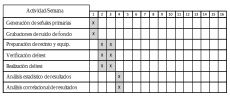
\includegraphics[width=\linewidth]{images/schedule.png}
\end{center}
\vspace{\captionSpace}
\begin{figure}[H]
    \caption{Cronograma detallado de las etapas y actividades del proyecto de investigación.}
    \label{fig:schedule}
\end{figure}

\section{Referencias}
\renewcommand{\refname}{}
\vspace{-3em}
\printbibliography

\end{document}
